\chapter{Soporte software del robot}
\label{cap:capitulo6}



\begin{flushright}
\begin{minipage}[]{10cm}
\emph{El software es una gran combinación entre arte e ingeniería}\\
\end{minipage}\\

Bill Gates\\
\end{flushright}

\vspace{1cm}
\setcounter{footnote}{84}

Una vez contado todo el proceso llevado a cabo para el diseño y construcción del prototipo robótico, en este capítulo se aborda el soporte \textit{software} en el robot para ponerlo en funcionamiento tanto en simulación como en la vida real.

\section{Simulación}
\label{sec:simulacion}

En esta sección se va a tratar el proceso seguido para conseguir poner a PiBotJ en funcionamiento a través de simulación, en concreto usando Gazebo. Esta parte ha sido desarrollada en el ordenador principal que se ha usado para este proyecto, explicado en el Apartado \ref{subsec:ordenador}, y por tanto, usa Ubuntu 22.04 \acs{LTS} y ROS 2 Humble. Para conseguir la simulación, ha sido necesario tener instalado ROS 2 Humble\footnote{\url{https://docs.ros.org/en/humble/Installation.html}} y seguir los siguientes pasos de instalación: 

\begin{verbatim}
	sudo apt update && sudo apt upgrade
	sudo apt install ros-humble-ros2-control ros-humble-ros2-controllers
	sudo apt install ros-humble-rviz2
	sudo apt install ros-humble-gazebo-ros-pkgs
	sudo apt install ros-humble-xacro ros-humble-robot-state-publisher 
	sudo apt install ros-humble-joint-state-publisher
\end{verbatim}

Una vez instalado todos los programas, fue el momento de empezar a desarrollar el código. 

\subsection{URDF/Xacro}
\label{subsec:urdf}

Primero de todo fue necesario definir las estructuras y propiedades del robot. Para ello, se decidió usar el formato \ac{URDF}\footnote{\url{http://wiki.ros.org/urdf}} y \textit{Xacro}\footnote{\url{http://wiki.ros.org/xacro}}, muy comunes en aplicaciones robóticas. \acs{URDF} usa un formato de ficheros XML y describe al robot como un conjunto de \textit{links} (enlaces), que están conectadas por una serie de \textit{joints} (articulaciones). Mientras que \textit{Xacro}, usa también un formato de ficheros XML que permite crear URDF de manera más modular, reutilizable y eficiente mediante el uso de macros y propiedades. Para más información se puede consultar la siguiente fuente\footnote{\url{https://articulatedrobotics.xyz/tutorials/ready-for-ros/urdf/}}.

En este proyecto se decidió crear una serie de ficheros \textit{Xacro}, cada uno dedicado a las distintas partes del robot (\verb|camera.xacro|\footnote{\url{https://github.com/RoboticsURJC/tfg-jlopez/blob/main/code/ros2/src/pibotj_r2c/description/camera.xacro}}, \verb|gps.xacro|\footnote{\url{https://github.com/RoboticsURJC/tfg-jlopez/blob/main/code/ros2/src/pibotj_r2c/description/gps.xacro}} y \verb|robot_core.xacro|\footnote{\url{https://github.com/RoboticsURJC/tfg-jlopez/blob/main/code/ros2/src/pibotj_r2c/description/robot_core.xacro}}). Cada fichero \textit{Xacro} necesita siempre tener la mismas etiquetas de \verb|<joint>| y \verb|<link>|, empleadas según convenga. Es importante tener en cuenta herramientas como validadores de XML\footnote{\url{https://www.xmlvalidation.com/index.php?id=1&L=0\#xml-9-6--1732781305}} para evitar problemas.

Existen cuatro tipos de \textit{joint}: \textit{prismatic}, \textit{continuous}, \textit{revolute} y \textit{fixed}. En el Código \ref{cod:fj} se puede ver la definición de una \textit{fixed joint}; si se quiere usar otro tipo de \textit{joint}, hay que añadir algunos campos\footnote{\url{https://articulatedrobotics.xyz/tutorials/ready-for-ros/urdf/\#joint-tags}}.

\begin{code}[h]
	\begin{lstlisting}[language=xml]
		<joint name="gps_joint" type="fixed">
			<parent link="chassis"/>
			<child link="gps_frame"/>
			<origin xyz="-0.1 0.0 0.04" rpy="0 0 0"/>
		</joint>
	\end{lstlisting}
	\caption[Macro que define \textit{fixed joint}]{Macro que define una \textit{fixed joint}}
	\label{cod:fj}
			\end{code}

En relación a los \textit{link}, obligatoriamente tienen que tener las macros de \verb|<visual>|, \verb|<collision>| e \verb|<inertial>|, sino pueden surgir errores\footnote{\url{https://answers.gazebosim.org//question/25166/problem-changing-joint-from-fixed-to-revolute/}}. Existen cuatro tipos de geometría: \textit{box}, \textit{cylinder}, \textit{sphere} y \textit{mesh}. El Código \ref{cod:ml} muestra un ejemplo de una \textit{mesh link} pero si se quiere tratar más ejemplos, se puede consultar la siguiente fuente\footnote{\url{https://articulatedrobotics.xyz/tutorials/ready-for-ros/urdf/\#link-tags}}.

\begin{code}[h]
	\begin{lstlisting}[language=xml]
		<link name="camera_link">
			<visual>
				<origin xyz="0.02 0.01 0.0 " rpy="0 0 ${-pi/2}"/>
				<geometry>
					<mesh filename="package://pibotj_r2c/meshes/camara.stl" scale="0.001 0.001 0.001"/>
				</geometry>
				<material name="Blue">
					<color rgba="${0/255} ${0/255} ${255/255} 1.0"/>
				</material>
			</visual>
			<collision> 
				<origin xyz="0.0 0.0 0.0 " rpy="0 0 ${-pi/2}"/>
				<geometry>
					<mesh filename="package://pibotj_r2c/meshes/camara.stl" scale="0.001 0.001 0.001"/>
				</geometry>
			</collision>
			<inertial>
				<origin xyz="0.0 0.0 0.0" rpy="0 0 ${-pi/2}"/>
				<mass value="0.03"/> <!--30g-->
				<inertia ixx="0.01" ixy="0.0" ixz="0.0" iyy="0.005" iyz="0.0" izz="0.005"/>
			</inertial>
		</link>
	\end{lstlisting}
	\caption[Macro que define una \textit{mesh link}]{Macro que define una \textit{mesh link}}
	\label{cod:ml}
\end{code}


Una vez fueron definidas las distintas partes del robot, fue el momento de incluir en los distintos ficheros las interacciones del robot con el simulador y para ello se usa la macro \verb|<gazebo>|. En el presente proyecto, se ha simulado el sensor cámara y el módulo \acs{GPS}. Existen muchos tipos de interacciones pero el Código \ref{cod:gazebo} muestra cómo simular el sensor cámara. Para simular el módulo GPS se ha utilizado un mensaje del tipo NavSatFix\footnote{\url{http://docs.ros.org/en/api/sensor_msgs/html/msg/NavSatFix.html}}. Si se quiere tratar más ejemplos, se puede consultar la siguiente fuente\footnote{\url{http://wiki.ros.org/urdf/XML/Gazebo}}.

\begin{code}[h]
	\begin{lstlisting}[language=xml]
		<gazebo reference="camera_link_optical">
		<material>Gazebo/Blue</material>
			<sensor name="camera" type="camera">
				<pose> 0 0 0 0 0 0 </pose>
				<visualize>true</visualize>
				<update_rate>10</update_rate>
				<camera>
					<horizontal_fov>1.089</horizontal_fov>
					<image>
						<format>R8G8B8</format>
						<width>640</width>
						<height>480</height>
					</image>
					<clip>
						<near>0.05</near>
						<far>8.0</far>
					</clip>
				</camera>
				<plugin name="camera_controller" filename="libgazebo_ros_camera.so">
					<frame_name>camera_link_optical</frame_name>
				</plugin>
			</sensor>
		</gazebo>
	\end{lstlisting}
	\caption[Macro que permite a Gazebo simular una cámara]{Macro que permite a Gazebo simular una cámara}
	\label{cod:gazebo}
\end{code}

En el presente proyecto se han definido los sistemas de coordenadas que aparecen en la Figura \ref{fig:links}. Una vez se definió el robot y los sensores necesarios para que Gazebo interactuara con el modelo, era el momento de usar ROS 2 Control. 

\begin{figure} [h!]
	\begin{center}
		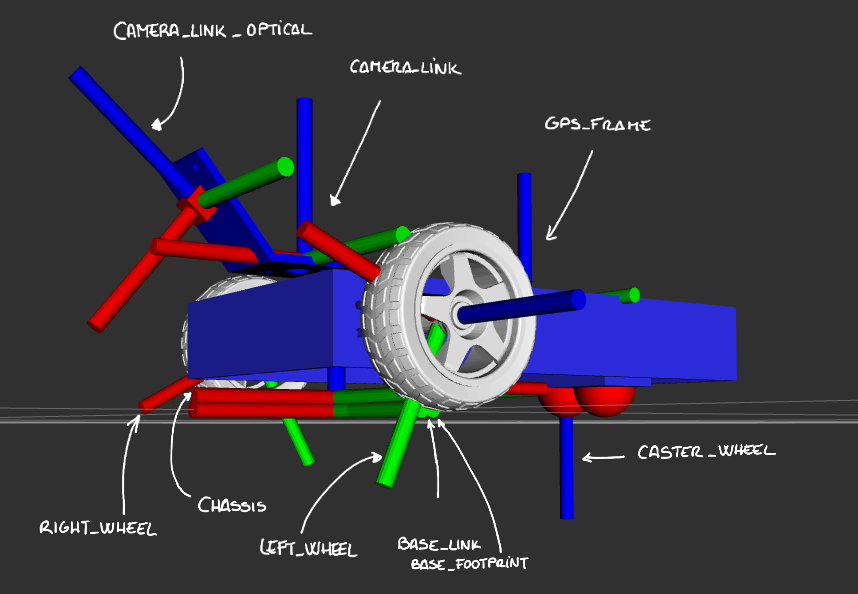
\includegraphics[width=13cm]{figs/cap6/links.png}
	\end{center}
	\caption{Sistemas de Coordenadas de PiBotJ}
	\label{fig:links}
\end{figure}


\subsection{ROS 2 Control}
\label{subsec:cap6ros2control}

Como se explicó en el Apartado \ref{subsec:ros2control}, ROS 2 Control es un \textit{framework} que permite gestionar y controlar los sensores y actuadores de manera eficiente y es por ello que se decidió aplicar a este proyecto a través del fichero \verb|ros2_control.xacro|\footnote{\url{https://github.com/RoboticsURJC/tfg-jlopez/blob/main/code/ros2/src/pibotj_r2c/description/ros2_control.xacro}}.

Este proyecto se definió un sistema llamado \textit{GazeboSystem} para el \textit{hardware interface}; de esta forma, es más sencillo añadir el número de sensores y actuadores que se necesiten. En este caso se decidió controlar a \textit{left\_wheel\_joint}, \textit{right\_wheel\_joint} y a \textit{camera\_joint}, que son aquellas \textit{joints} que tenían asignados en la vida real un motor. 

Si se ejecuta: \verb|ros2 control list_hardware_interfaces|, se puede ver las interfaces asociadas de lectura/escritura y de monitorización que tiene cada \textit{joint} a controlar. En la figura \ref{fig:ros2control} se puede ver las interfaces que tiene PiBotJ y por ende, cómo se van a controlar cada interfaz.

 \begin{figure} [h!]
 	\begin{center}
 		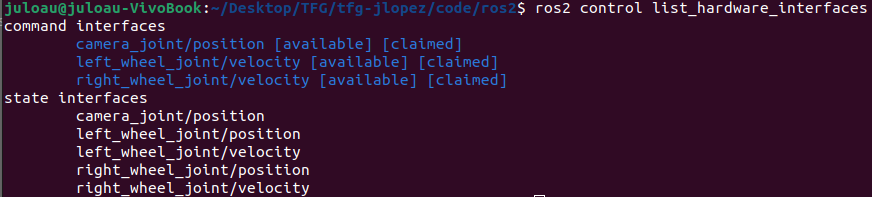
\includegraphics[width=14cm]{figs/cap6/interfaces.png}
 	\end{center}
 	\caption{Interfaces que tiene definidas PiBotJ}
 	\label{fig:ros2control}
 \end{figure}

Tras definir las \textit{joints} a controlar, era necesario definir en un fichero YAML, el tipo de controladores que utilizaba el \textit{controller manager}. Dentro de cada controlador, había que asignar las \textit{joints} definidas previamente al controlador que necesite cada una. En este caso, se asignaron las ruedas a un control diferencial y la cámara se decidió controlar por posición, usando el topic: \verb|\pos_cont|. Para más información, se puede consultar la siguiente fuente\footnote{\url{https://control.ros.org/humble/index.html}}.

Una vez el robot estaba completamente definido en los diferentes ficheros \textit{Xacro}, era necesario unirlos todos en otro fichero llamado \verb|robot.urdf.xacro|\footnote{\url{https://github.com/RoboticsURJC/tfg-jlopez/blob/main/code/ros2/src/pibotj_r2c/description/robot.urdf.xacro}} para poder facilitar el publicar el estado del robot y eso se consigue usando \verb|robot_state_publisher|.
 
\subsection{Robot State Publisher}
\label{subsec:robotstatepublisher}

En la Web oficial de ROS\footnote{\url{http://wiki.ros.org/robot_state_publisher}} se explica que \verb|robot_state_publisher| es esencial para publicar las transformaciones (tf) entre los diferentes \textit{links} del robot y para proporcionar información sobre el estado de sus \textit{joints} a cualquier componente en el sistema. Aunque pueda parecer complicado, la Figura \ref{fig:rsp}, obtenida de la web de Articulated Robotics\footnote{\url{https://articulatedrobotics.xyz/tutorials/mobile-robot/concept-design/concept-urdf\#quick-recap}}, resume muy bien los pasos que sigue \verb|robot_state_publisher|.

 \begin{figure} [h!]
	\begin{center}
		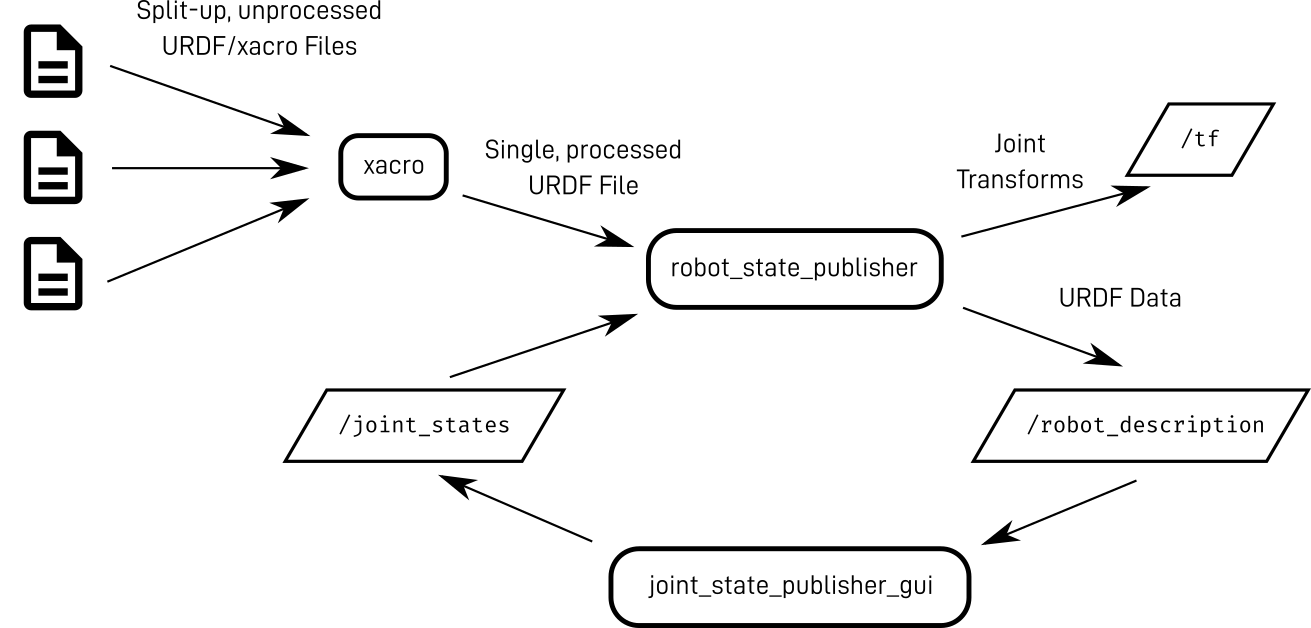
\includegraphics[width=12cm]{figs/cap6/rsp.png}
	\end{center}
	\caption{Diagrama de robot\_state\_publisher}
	\label{fig:rsp}
\end{figure}

Una vez todos los elementos a utilizar estaban listos, era el momento de aglutinarlos todos y crear un launcher que los inicializara y los pusiera en ejecución.

\subsection{Launcher}
\label{subsec:launcher}

El \textit{launcher} que se decidió crear para este proyecto parte del creado por Johnewans\footnote{\url{https://github.com/joshnewans/articubot_one/blob/main/launch/launch_sim.launch.py}}, creador de Articulated Robotics y fue modificado según las necesidades, siendo finalmente el resultante \verb|launch_sim.launch.py|\footnote{\url{https://github.com/RoboticsURJC/tfg-jlopez/blob/main/code/ros2/src/pibotj_r2c/launch/launch_sim.launch.py}}. Para facilitar su entendimiento, la Figura \ref{fig:launcherdiagram} explica los componentes que forman parte del \textit{launcher}. Llegados a este punto, PiBotJ ya estaba listo para ejecutarse completamente.


 \begin{figure} [h!]
	\begin{center}
		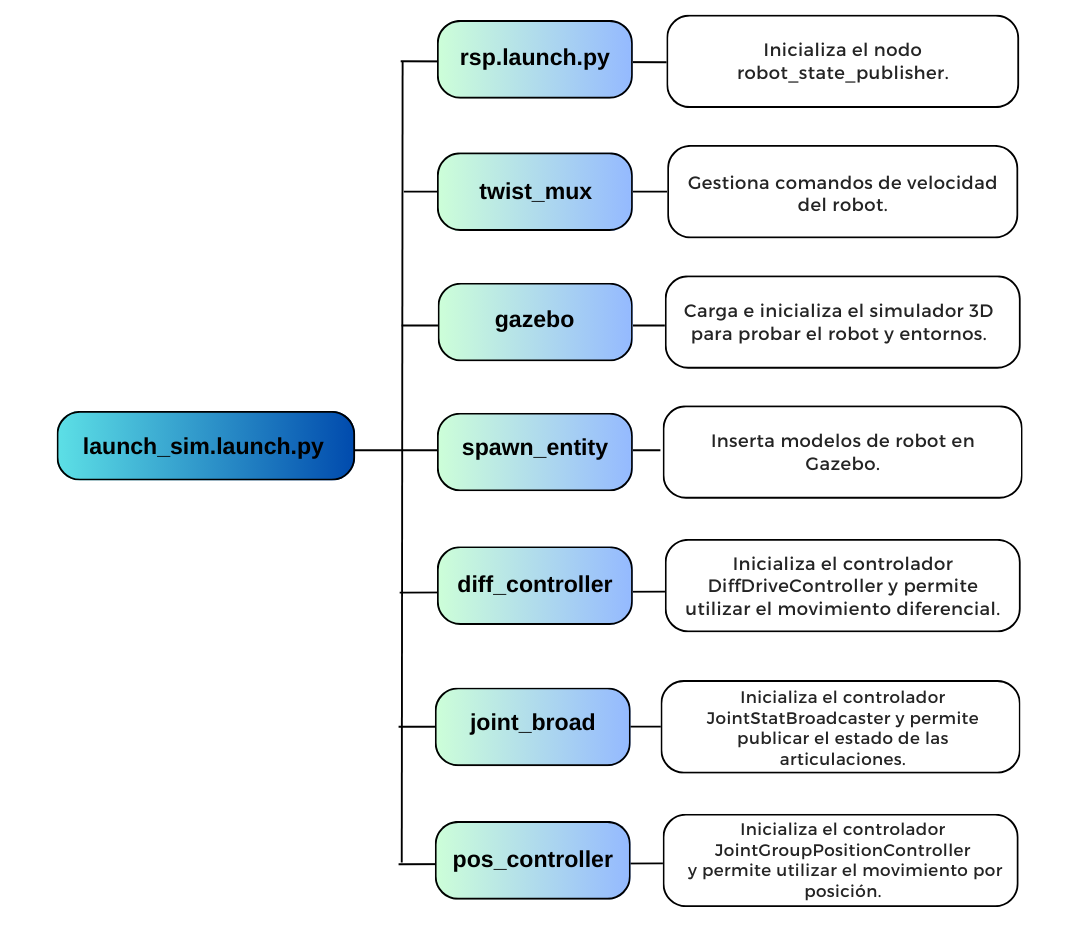
\includegraphics[width=14cm]{figs/cap6/diagram.png}
	\end{center}
	\caption{Esquema de launch\_sim.launch.py}
	\label{fig:launcherdiagram}
\end{figure}


\subsection{Simulación puesta en funcionamiento}
\label{subsec:funsimulacion}

Para poner en funcionamiento el modelo, únicamente había que escribir los siguientes comandos:
\begin{verbatim}
	colcon build --packages-select pibotj_r2c   # compila los paquetes
	source ./install/setup.bash                 # configura variables 
	ros2 launch pibotj_r2c launch_sim.launch.py
\end{verbatim} 

Si la primera vez que se lance el robot ocurre algún error, es normal y hay que reiniciar el proceso. Para demostrar que todos los topics que forman parte del robot se han inicializado correctamente, hay que escribir el siguiente comando:  \verb|ros2 topic list| y su salida se puede ver en la Figura \ref{fig:topic}.

 \begin{figure} [h!]
	\begin{center}
		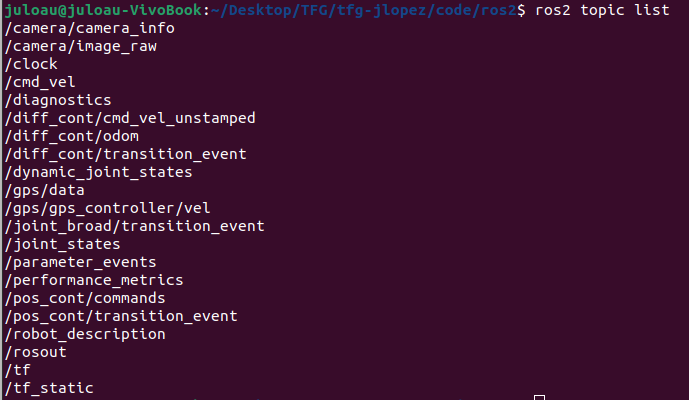
\includegraphics[width=12cm]{figs/cap6/topic.png}
	\end{center}
	\caption{Topics disponibles al lanzar el robot}
	\label{fig:topic}
\end{figure}


De todos esos topics, para poder conseguir el objetivo propuesto en la Sección \ref{sec:descripcion}, es necesario únicamente utilizar \verb|/camera/image_raw| para ver la imagen de la cámara, \verb|/cmd_vel| para mover las ruedas, \verb|/gps/data| para ver los valores de posición del \acs{GPS}, y \verb|/pos_cont/commands| para mover el motor de la cámara.

Para mover las ruedas hay muchas formas de hacerlo pero en este caso se usó \verb|rqt_robot_steering|, como muestra la Figura \ref{fig:steering}. Si se quiere visualizar la cámara, se puede usar \verb|rviz2| o \verb|ros2 run rqt_image_view rqt_image_view| que fue el comando usado para probar su funcionamiento (Figura \ref{fig:rqtimage}). Por otro lado, el módulo \acs{GPS} se puede visualizar sus valores usando \verb|ros2 topic echo /gps/data|, como muestra la Figura \ref{fig:echogps}. Finalmente para mover el motor de la cámara por posición, es necesario usar el comando: 

\begin{verbatim}
	ros2 topic pub /pos_cont/commands std_msgs/msg/Float64MultiArray \
	 "data: [-0.5]"
\end{verbatim} 

Siendo los valores que van dentro de data desde 3 (giro hacia la izquierda) hasta -3 (giro hacia la derecha). En la Figura \ref{fig:camararot} se pueden ver los dos casos descritos previamente. 


 \begin{figure} [h!]
	\begin{center}
		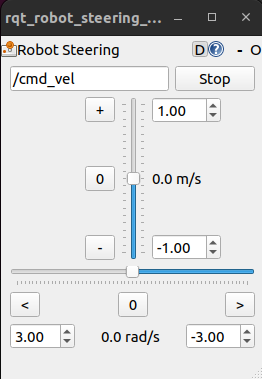
\includegraphics[width=6cm]{figs/cap6/steering.png}
	\end{center}
	\caption{Herramienta usada para mover las ruedas}
	\label{fig:steering}
\end{figure}

 \begin{figure} [h!]
	\begin{center}
		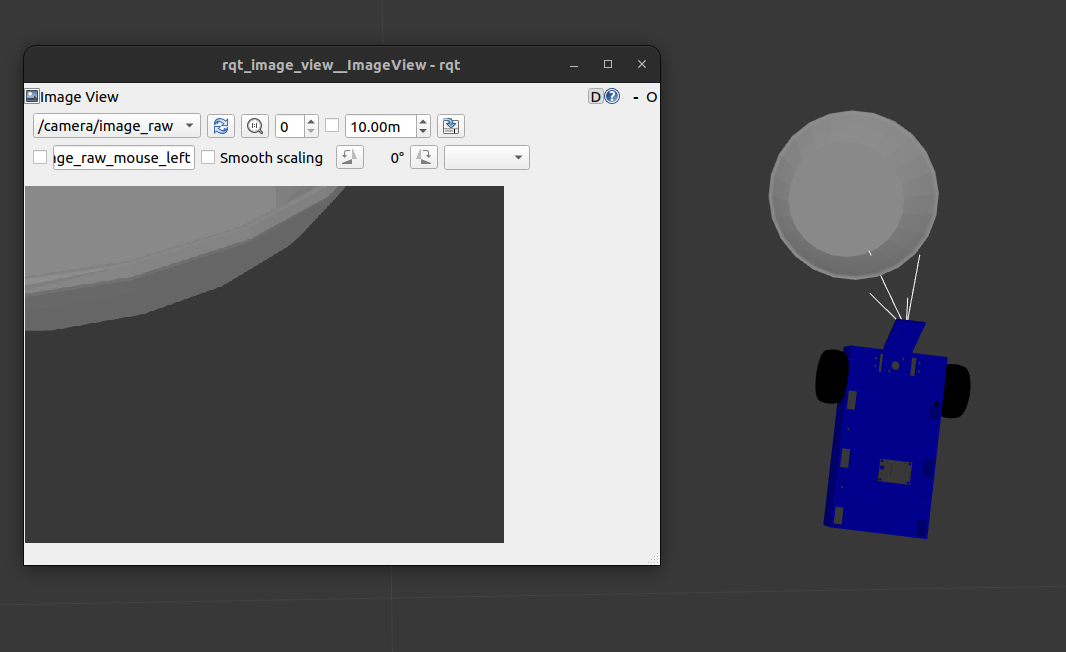
\includegraphics[width=12cm]{figs/cap6/rqtimage.png}
	\end{center}
	\caption{Herramienta usada para visualizar la cámara}
	\label{fig:rqtimage}
\end{figure}

 \begin{figure} [h!]
	\begin{center}
		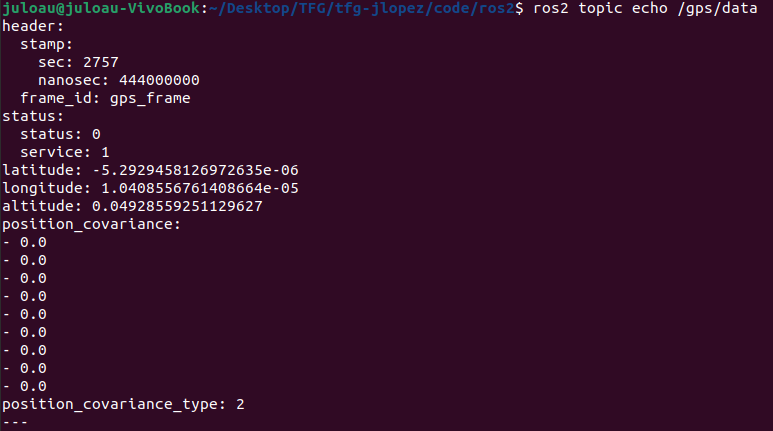
\includegraphics[width=12cm]{figs/cap6/echogps.png}
	\end{center}
	\caption{Herramienta usada para visualizar los valores del GPS}
	\label{fig:echogps}
\end{figure}


\begin{figure}[ht!]
	\centering
	\begin{minipage}{0.45\linewidth}
		\centering
		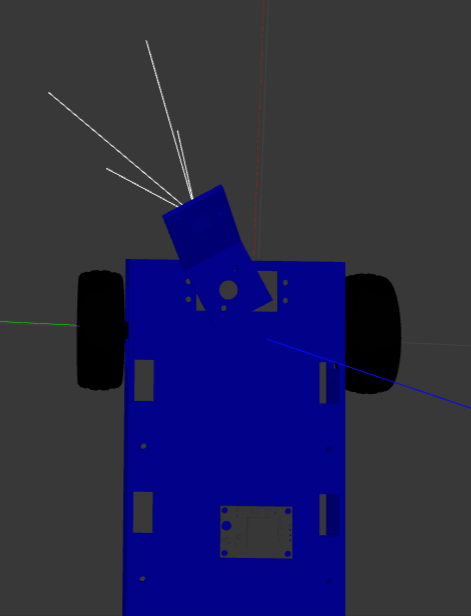
\includegraphics[width=\linewidth]{figs/cap6/rotizq.png}
		\caption*{\centering Rotación hacia la izquierda} 
	\end{minipage}
	\hspace{0.25cm}
	\begin{minipage}{0.45\linewidth}
		\centering
		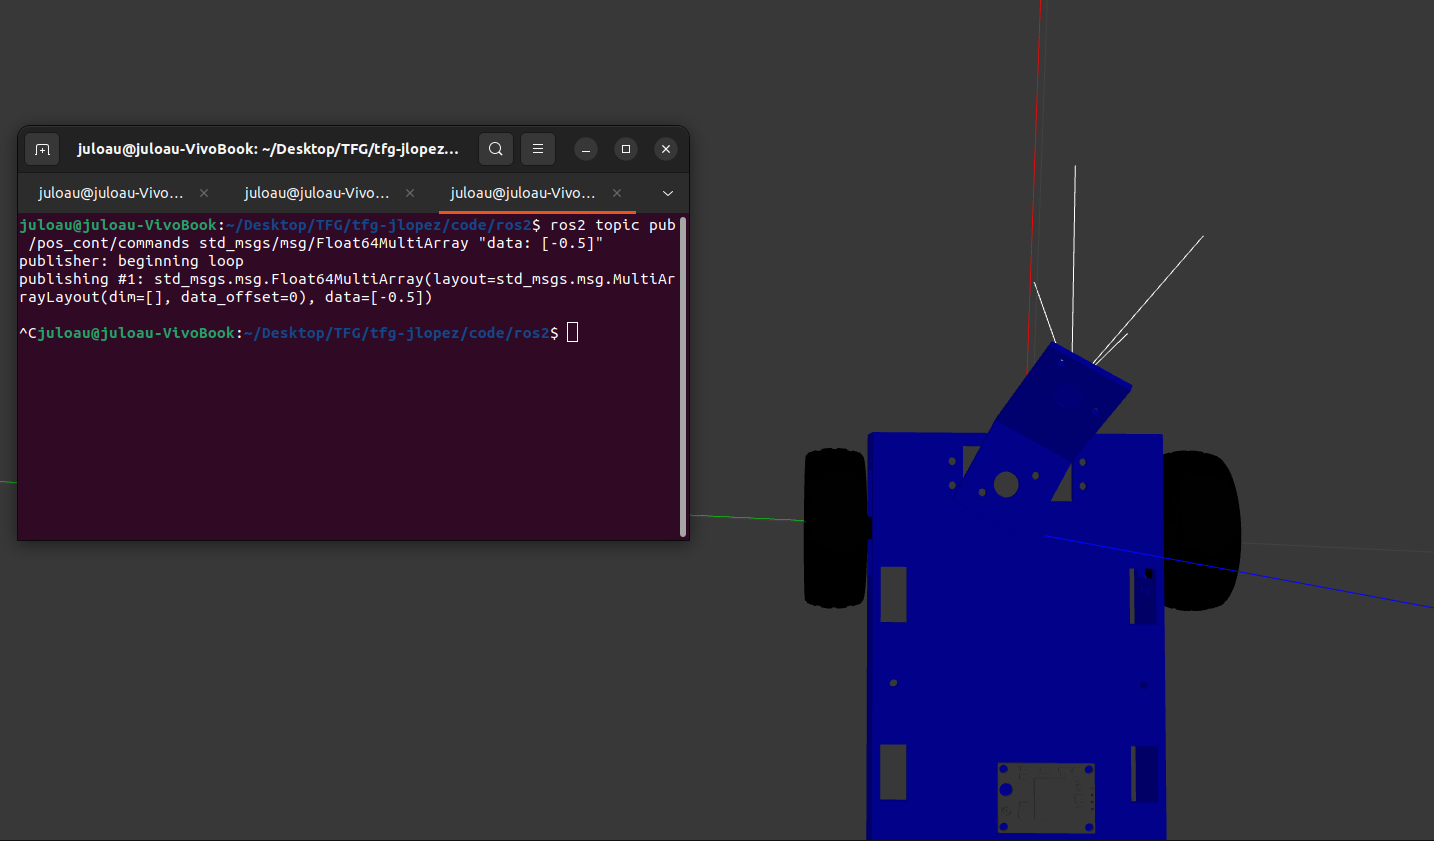
\includegraphics[width=\linewidth]{figs/cap6/rotder.png}
		\caption*{\centering Rotación hacia la derecha} 
	\end{minipage}
	\caption{Herramienta usada para rotar la cámara}
	\label{fig:camararot}
\end{figure}


Una vez se ha demostrado el funcionamiento de PiBotJ en simulación con este video\footnote{\url{https://www.youtube.com/watch?v=A0yi7YlLpq0}}, ya se puede dar soporte al robot físico.

\section{Configuración del robot físico}
\label{sec:configrf}

Como se explicó en la sección anterior, el robot ya estaba listo en simulación para, a través de los topics definidos en el apartado anterior, poder definir y monitorear su comportamiento. Después de eso, era momento de poner al robot físico también listo para operar.    

En la Raspberry Pi se decidió instalar Ubuntu 20.04 Server \acs{LTS}, como se explicó en el Apartado \ref{subsec:ubuntu}, y para ello, fue necesario instalar en el ordenador principal, que actuaba como cliente, el siguiente programa:  \verb|sudo apt-get install openssh-client|. Como en Ubuntu 20.04 la distribución de ROS 2 era foxy, había que seguir los pasos de instalación de la Sección \ref{sec:simulacion} pero cambiando humble por foxy. 

Por otro lado, ahora desde una terminal del ordenador, se puede conectar al robot a través de ssh, escribiendo \verb|ssh usuario@ip_dispositivo| y posteriormente, introduciendo la constraseña creada en el proceso de instalación. Esta era la forma de comunicación con el robot ya que esta distribución, no tenía interfaz gráfica. De las variante de ssh se usaba scp -r para copiar directorios entre el robot y el ordenador local y permitir subir los cambios a Github, y para desarrollar código se usaba un \textit{plugin} de VSCode que permite usar VSCode conectándose al robot usando ssh\footnote{\url{https://code.visualstudio.com/docs/remote/ssh-tutorial}}. 

Es importante recordar que al usar ROS 2, todos los nodos que estén ejecutando dentro de una red Wifi, serán visibles para cualquier dispositivo que esté conectado dentro de esa red Wifi. Gracias a eso, se facilitó la depuración y monitorización de cada sensor y actuador de PiBotJ. 

Una vez dentro del robot y conociendo todas las posibles formas de estar comunicados con él, era el momento de configurar cada dispositivo que conformaba a PiBotJ.

\subsection{Cámara}
\label{subsec:configcamara}

La cámara fue conectada en el puerto CSI y para hacerla funcionar fue necesario instalar los siguientes programas: 

\begin{verbatim}
	sudo apt-get install gstreamer1.0-tools \ 
	gstreamer1.0-plugins-base gstreamer1.0-plugins-good \ 
	gstreamer1.0-plugins-bad gstreamer1.0-plugins-ugly
\end{verbatim}

Una vez instalados, fue necesario editar el fichero \verb|/boot/firmware/config.txt| añadiendo \verb|start_x=1| al final y se tuvo que reiniciar la Raspberry Pi. Para comprobar que la configuración fue correcta, era necesario usar el comando \verb|v4l2-ctl --list-devices|  que comprueba la lista de dispositivos de video y media que están disponibles en el sistema. En la Figura \ref{fig:v4l2} se puede ver el resultado de dicho comando y  muestra que la cámara se encontraba conectada en el dispositivo \verb|/dev/video0|.

 
 \begin{figure} [h!]
	\begin{center}
		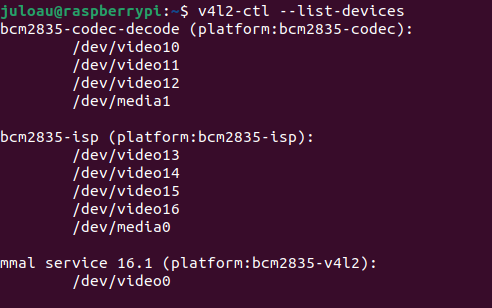
\includegraphics[width=9cm]{figs/cap6/vl.png}
	\end{center}
	\caption{Dispositivos de video y media disponibles en PiBotJ}
	\label{fig:v4l2}
\end{figure}


Sabiendo que la cámara estaba disponible, era necesario comprobar que realmente la imagen se pudiera ver correctamente. Para ello, partiendo del \verb|cameraPublisher.py| de este tutorial\footnote{\url{https://www.youtube.com/watch?v=6e94ZnYnO_U}}, se pudo crear un nodo llamado \verb|camera_node|\footnote{\url{https://github.com/RoboticsURJC/tfg-jlopez/blob/main/code/ros2/src/pibotj_rr/pibotj_rr/camera.py}} que permitía leer y publicar la imagen del dispositivo de la cámara. Se podía monitorizar usando las mismas herramientas que en el Apartado \ref{subsec:funsimulacion} para controlar la cámara en simulación (Figura \ref{fig:camararr}).

 \begin{figure} [h!]
	\begin{center}
		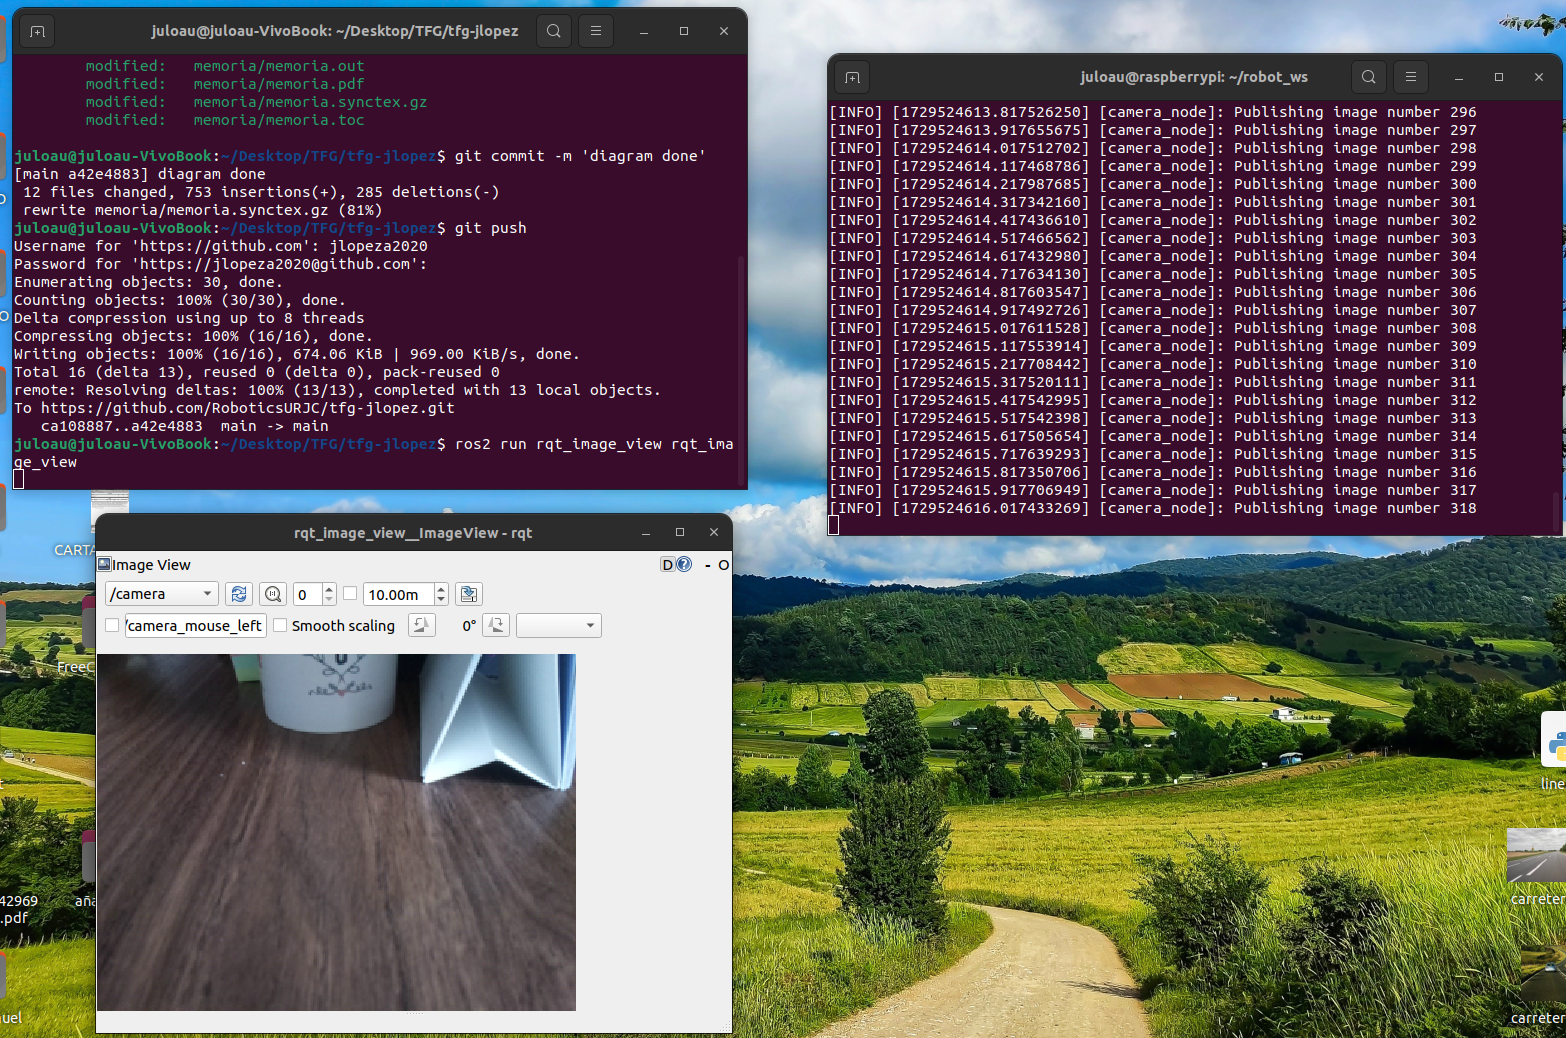
\includegraphics[width=12cm]{figs/cap6/camerarr.png}
	\end{center}
	\caption{Cámara de PiBotJ en funcionamiento}
	\label{fig:camararr}
\end{figure}

Para posteriores cálculos, era necesario conocer tanto los parámetros intrínsecos como extrínsecos de la cámara.  

\subsubsection{Parámetros intrínsecos}
\label{subsubsec:intrinsecoscamara}

Los parámetros intrínsecos definen la geometría interna y la óptica de la cámara. Estos determinan cómo la cámara proyecta los puntos del mundo 3D al plano de la imagen en 2D, siendo constantes en tanto no varíen las características y posiciones relativas entre la óptica y el sensor imagen. Estos parámetros los provee el fabricante de la cámara, o bien se pueden estimar, y se decidió calcular las dos posibles opciones.

Para los cálculos teóricos se decidió consultar en numerosas fuentes de información y gracias a \textit{Elinux}\footnote{\url{https://elinux.org/Rpi_Camera_Module\#Technical_Parameters_.28v.2_board.29}} se pudo obtener sus parámetros técnicos y partiendo del libro \cite{Hartley2004} (final paǵina 156 y principio de la página 157) y cálculos básicos matemáticos, se pudo encontrar las fórmulas de la distancia focal (Ecuación \ref{ec:distfocal}) y del centro de la imagen (Ecuación \ref{ec:cenimagen}).


\begin{myequation}[h]
	\begin{align}
		f_x &= F \cdot \frac{\text{Res. horizontal}}{\text{tam. sensor horizontal}} \quad
		f_x = 3.04 \cdot \frac{640}{3.674} = 529,56 \\
		\hspace{1cm}
		f_y &= F \cdot \frac{\text{Res. vertical}}{\text{tam. sensor vertical}} \quad
		f_y = 3.04 \cdot \frac{480}{2.760} = 528,69
	\end{align}
	\caption[Fórmula para calcular la distancia focal teórica]{Fórmula para calcular la distancia focal teórica}
	\label{ec:distfocal}
\end{myequation}

\begin{myequation}[h]
	\begin{align}
		c_x &= \frac{\text{Res. horizontal}}{2} \quad
		c_x = \frac{640}{2} = 320 \\
		\hspace{1cm}
		c_y &= \frac{\text{Res. vertical}}{2} \quad
		c_y =  \frac{480}{2} = 240
	\end{align}
	\caption[Fórmula para calcular el centro de la imagen]{Fórmula para calcular el centro de la imagen}
	\label{ec:cenimagen}
\end{myequation}


Para los cálculos prácticos, ha sido necesario seguir los pasos de calibración creando los ficheros de \verb|calibration.py|\footnote{\url{https://github.com/RoboticsURJC/tfg-jlopez/blob/main/code/camera/calibration/calibration.py}} y \verb|process.py|\footnote{\url{https://github.com/RoboticsURJC/tfg-jlopez/blob/main/code/camera/calibration/process.py}} partiendo del tutorial\footnote{\url{https://www.youtube.com/watch?v=XFBKwme5HYk}}. El fichero \verb|calibration.py| capturaba las imágenes con el patrón de ajedrez y el fichero \verb|process.py| generaba la matriz de parámetros intrínsecos y de distorsión. El proceso se repitió diez veces y finalmente la matriz resultante fue la media de las diez matrices de parámetros intrínsecos y sus valores se muestran en la Figura \ref{fig:meanintrinseco}. Los valores son: $f_x$ = 497,66 , $f_y$ = 502,16 , $c_x$ = 325,3 y $c_y$ = 240,18

 \begin{figure} [h!]
	\begin{center}
		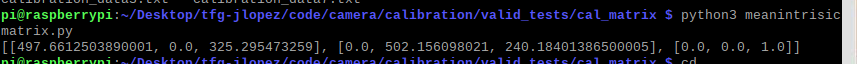
\includegraphics[width=15cm]{figs/cap6/intrinsicmedia.png}
	\end{center}
	\caption{Media de la matriz de intrínsecos}
	\label{fig:meanintrinseco}
\end{figure}


Podemos ver que los valores teóricos difieren de la realidad y es debido a que existen muchos factores que pueden influir y aunque el fabricante decida poner unos valores, cada cámara termina teniendo los suyos propios, creando un margen de error.


\subsubsection{Parámetros extrínsecos}
\label{subsubsec:extrinsecoscamara}

Los parámetros extrínsecos relacionan los sistemas de referencia del mundo real y la cámara, describiendo la posición y orientación de la cámara en el sistema de coordenadas del mundo real. Dichos parámetros engloban la rotación y la traslación de la cámara. En este caso la cámara tiene una rotación sobre el eje Y de 50º (Figura \ref{fig:extrinseco} izquierda) y está trasladada 8,8 cm en el eje Z (Figura \ref{fig:extrinseco} derecha). 

\begin{figure}[ht!]
	\centering
	\begin{minipage}{0.45\linewidth}
		\centering
		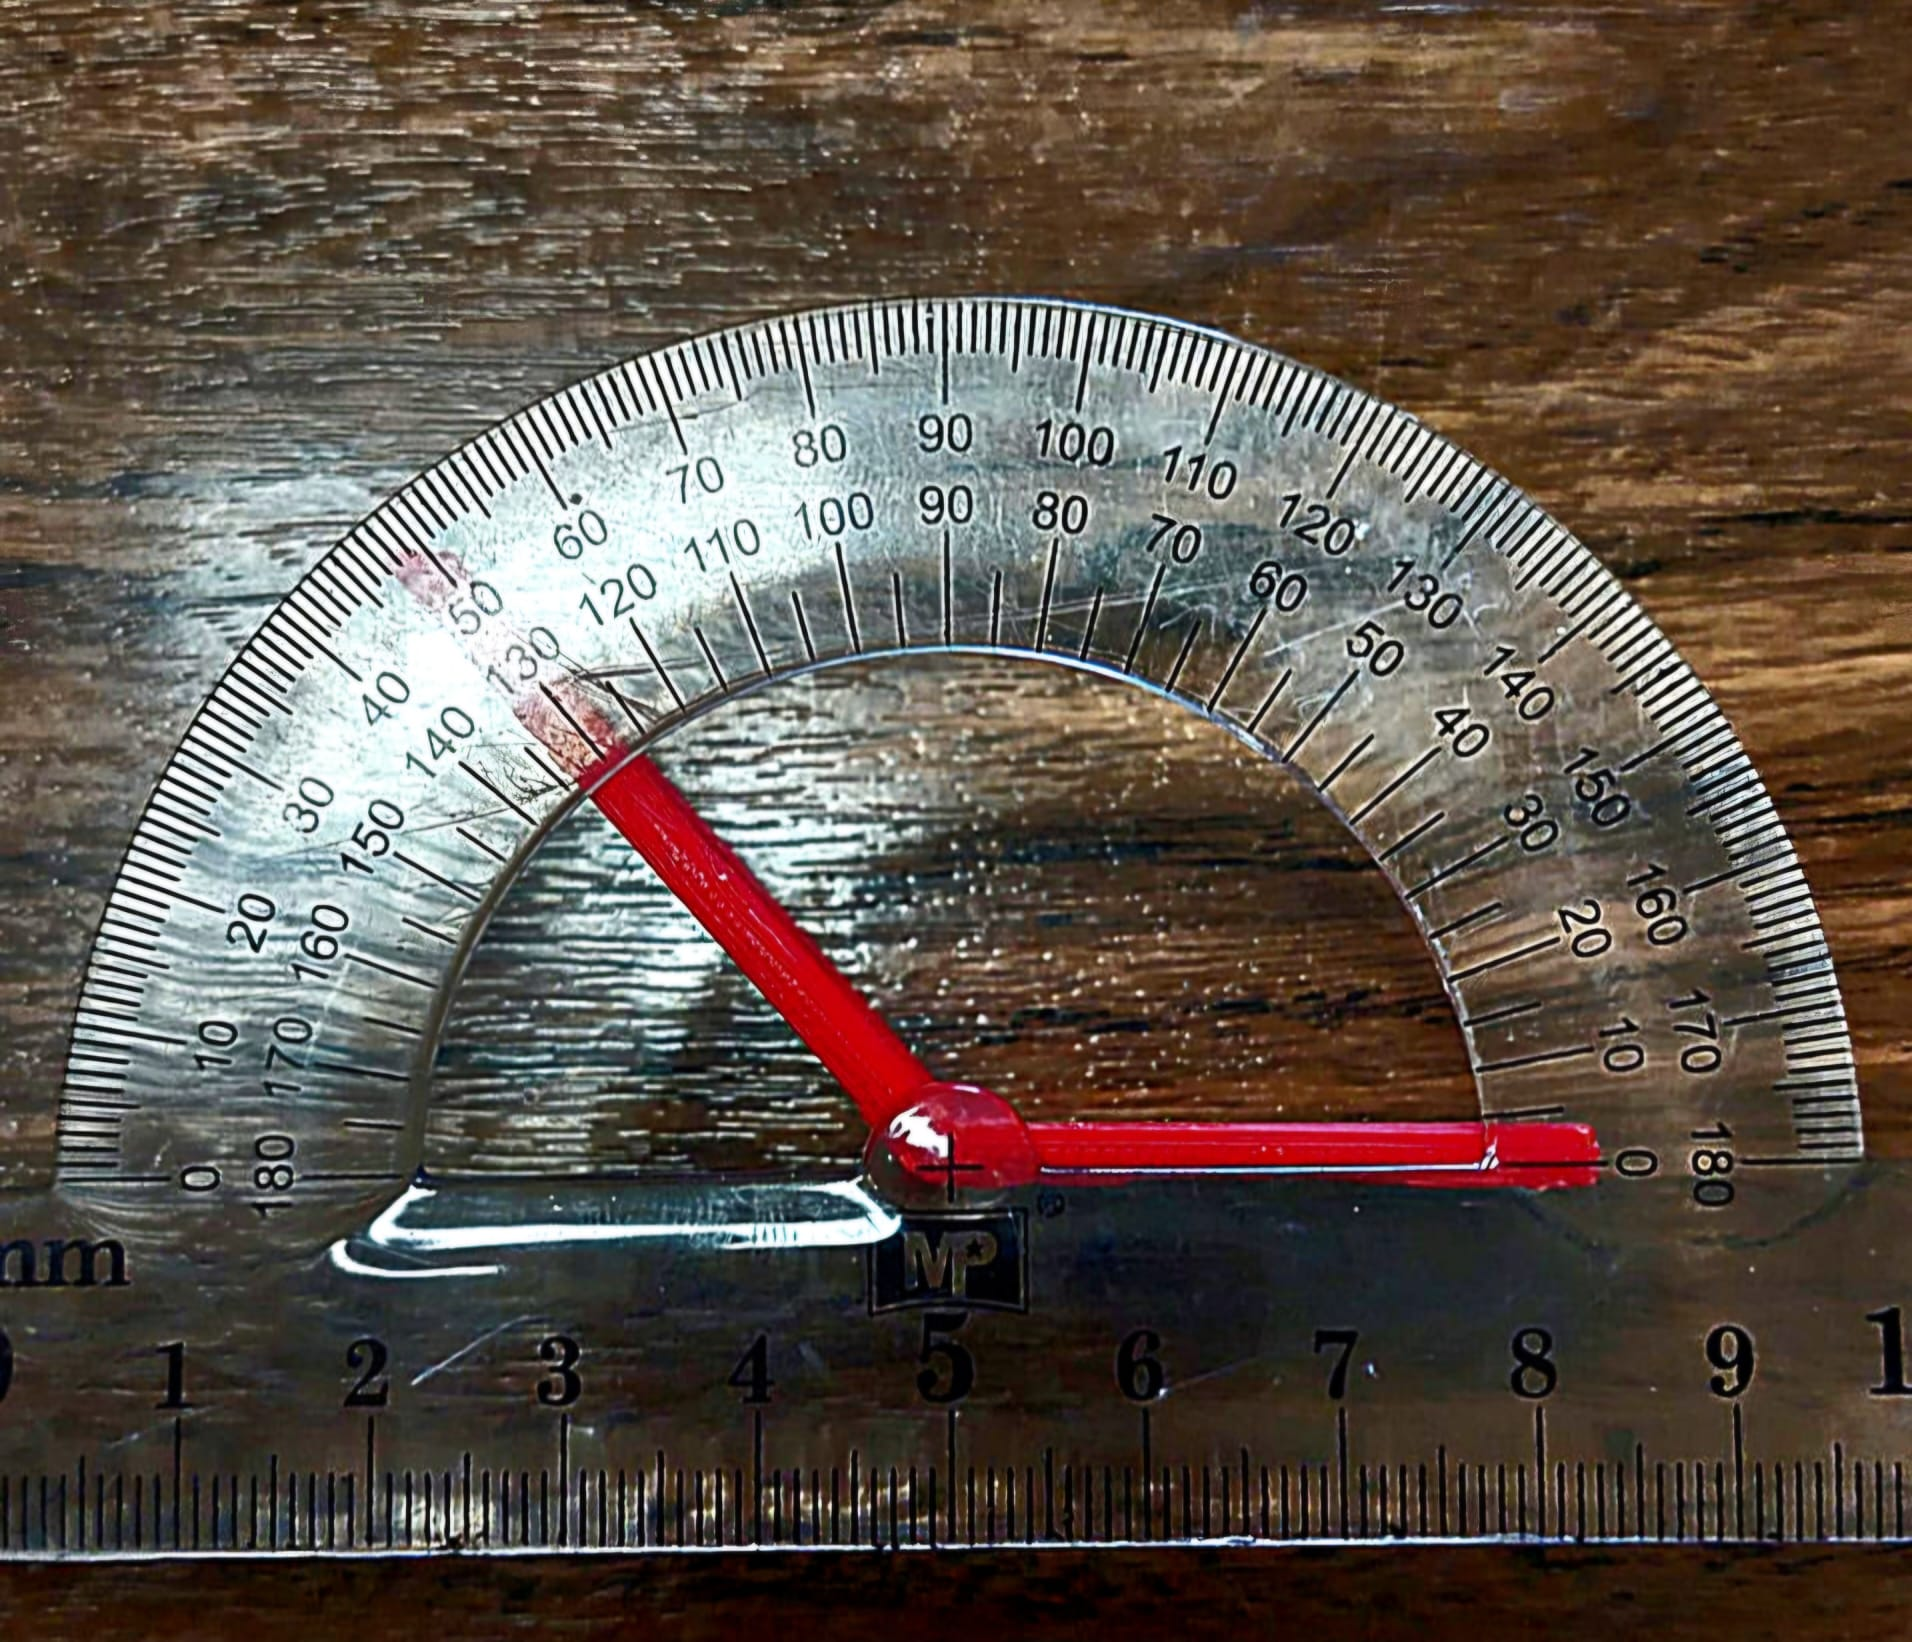
\includegraphics[width=\linewidth]{figs/cap6/rotation.jpeg}
		\caption*{\centering Rotación de la cámara} 
	\end{minipage}
	\hspace{0.25cm}
	\begin{minipage}{0.45\linewidth}
		\centering
		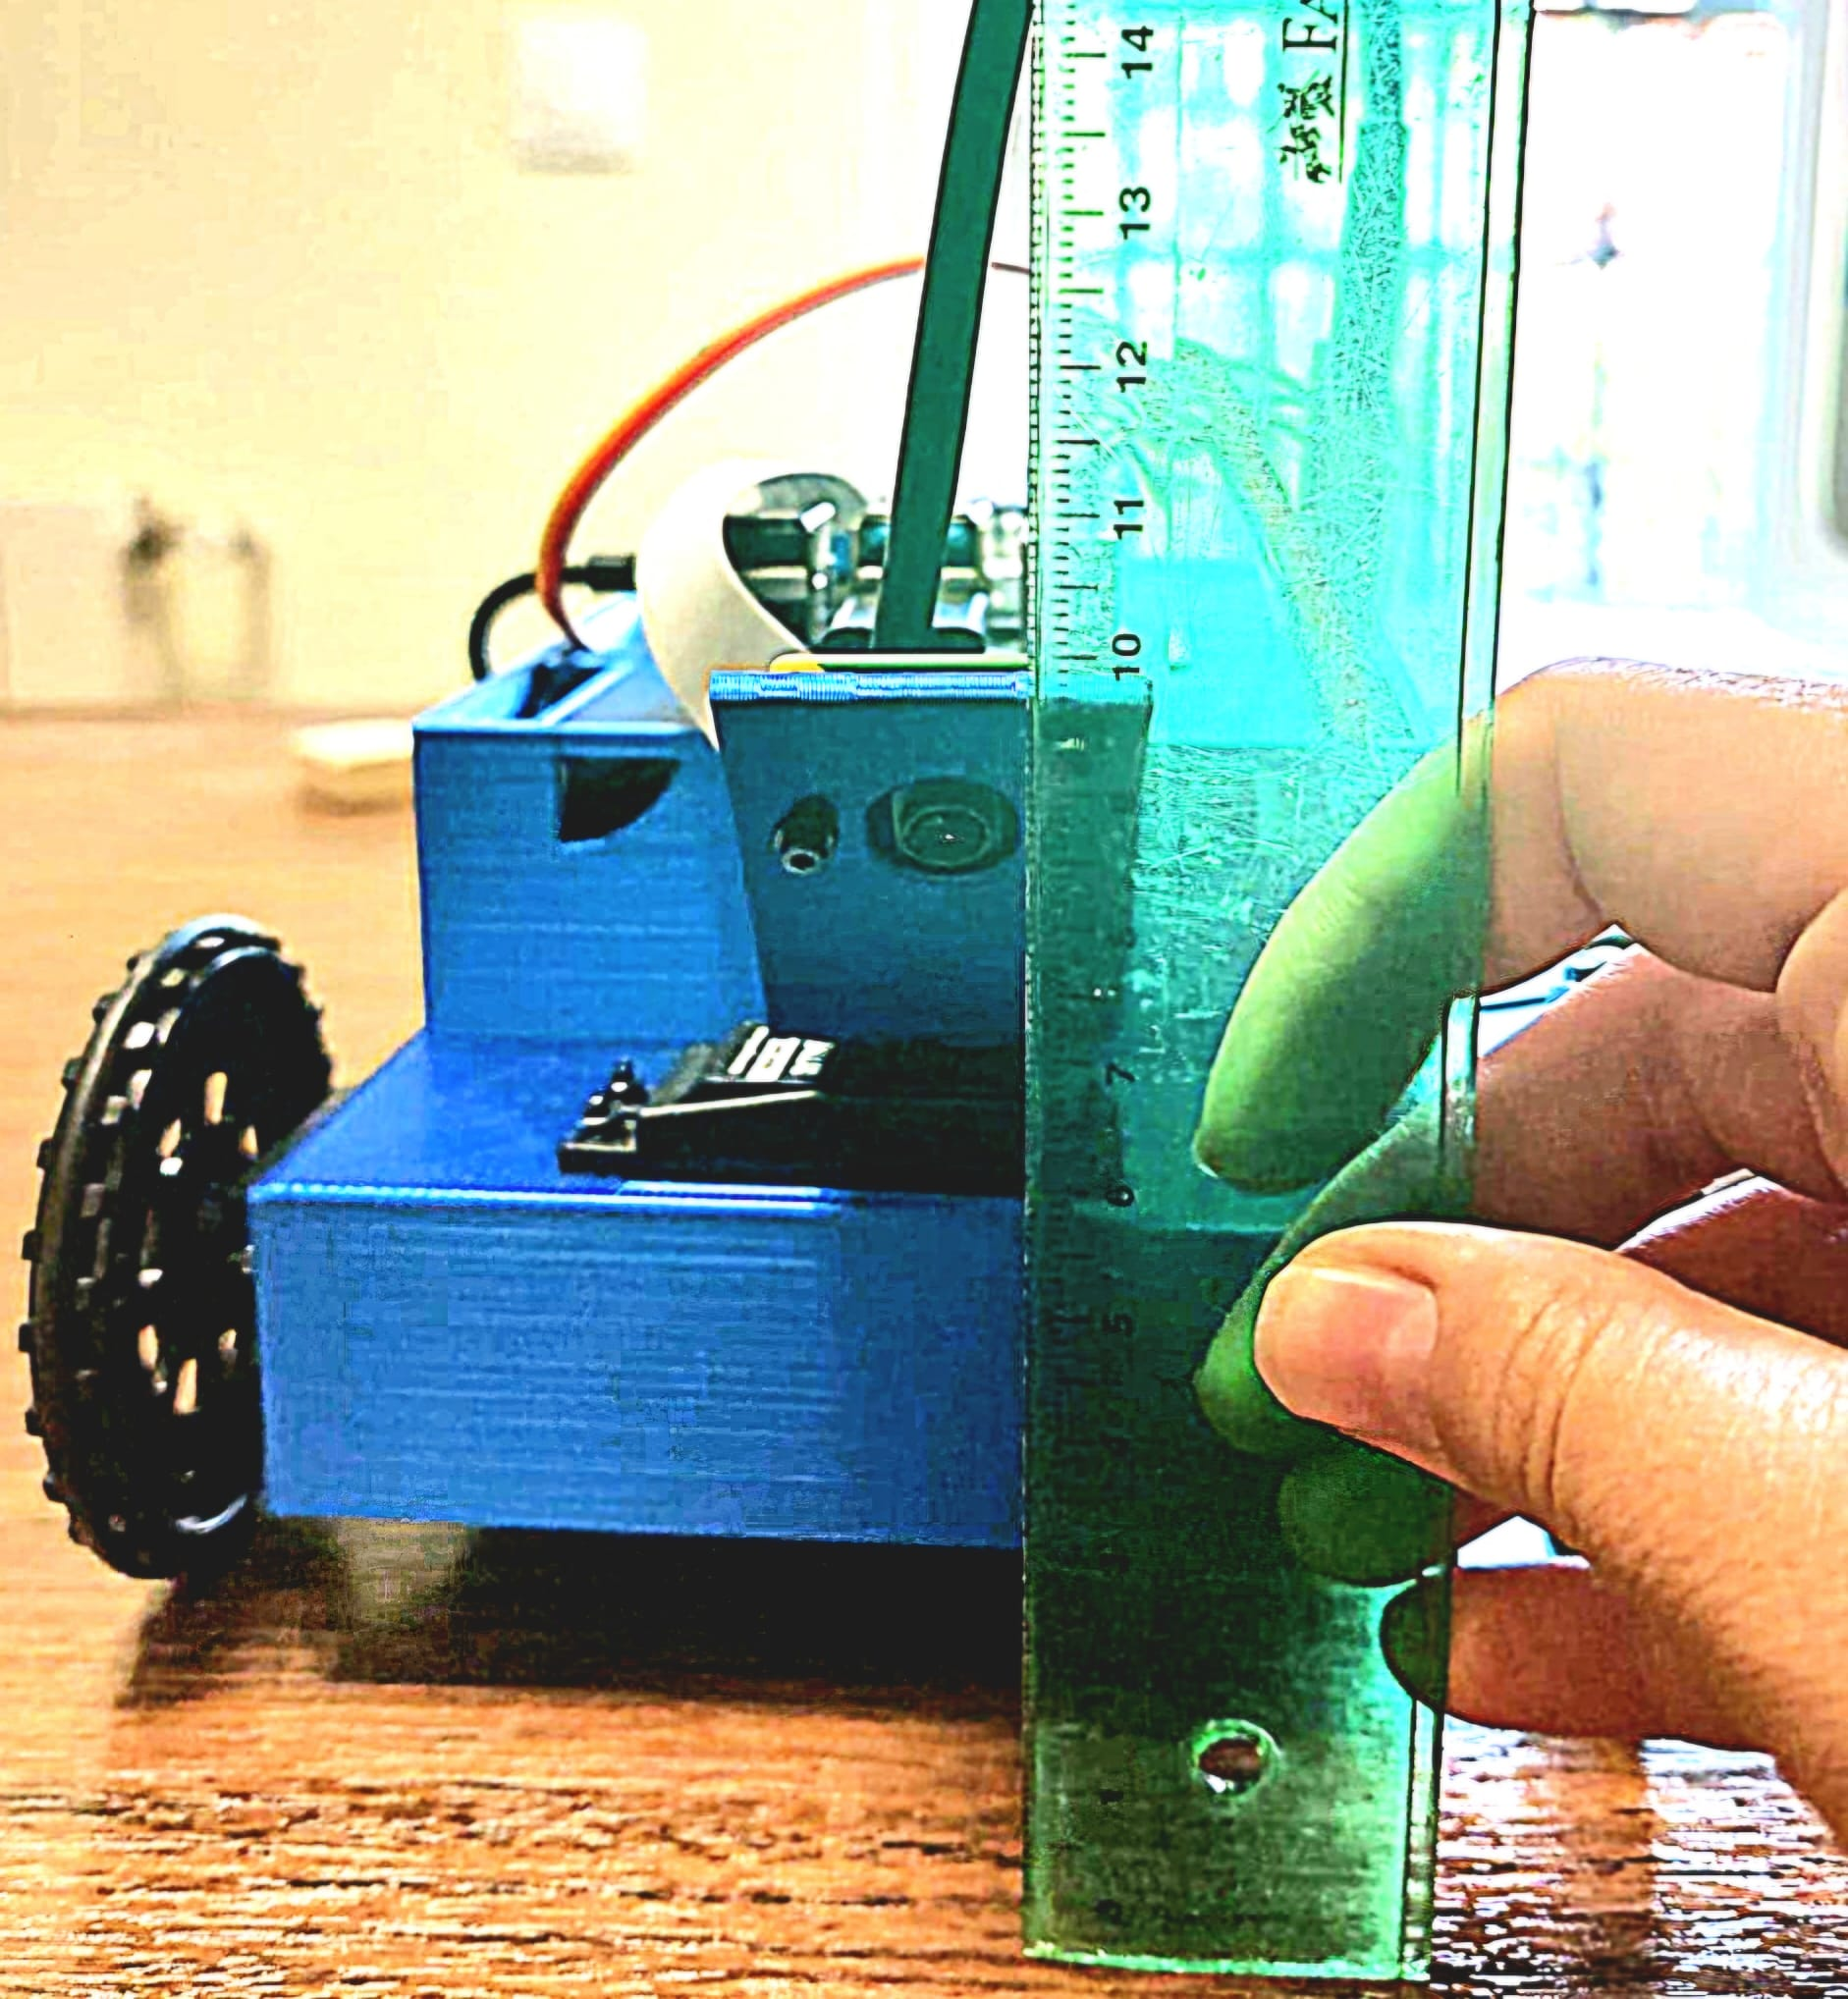
\includegraphics[width=\linewidth]{figs/cap6/traslacion.jpeg}
		\caption*{\centering Traslación de la cámara} 
	\end{minipage}
	\caption{Parámetros extrínsecos}
	\label{fig:extrinseco}
\end{figure}


\subsection{Google Coral USB}
\label{subsec:configgcoral}

Una vez la cámara estaba lista para operar y se conoce que existen muchas limitaciones cuando se trata de acelerar tareas en dispositivos que no cuentan con \textit{hardware} para ello, como se comentó en el Apartado \ref{subsec:googlecoral}, se decidió incluir el dispositivo USB Google Coral y para ello, es necesario configurarlo.

En su web oficial\footnote{\url{https://coral.ai/docs/accelerator/get-started/}} se pueden encontrar diferentes pasos de instalación dependiendo de las necesidades del usuario, pero se pueden resumir para cumplir con las características de la arquitectura de este dispositivo de la siguiente manera:


\begin{lstlisting}[language=bash]
 echo "deb https://packages.cloud.google.com/apt \
 coral-edgetpu-stable main" | \
 sudo tee /etc/apt/sources.list.d/coral-edgetpu.list

 curl https://packages.cloud.google.com/apt/doc/apt-key.gpg \
  | sudo apt-key add -

 sudo apt-get update	

 sudo apt-get install libedgetpu1-std

 # Conecta el USB en uno de los puertos 3.0

 sudo apt-get install python3-pycoral
\end{lstlisting}

Finalmente, el proceso se debería haber completado cuando la salida del último comando se debería ver como muestra la Figura \ref{fig:outcoral}.

 \begin{figure} [h!]
	\begin{center}
		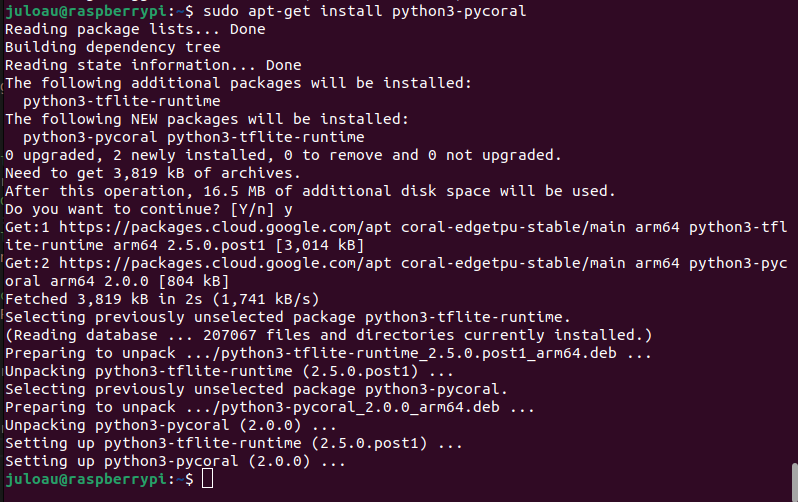
\includegraphics[width=12cm]{figs/cap6/pycoralinstalled.png}
	\end{center}
	\caption{Configuración exitosa del Google Coral}
	\label{fig:outcoral}
\end{figure}


\subsection{Módulo GPS}
\label{subsec:configgps}

El módulo \acs{GPS} utiliza una comunicación \ac{UART}, o también conocido como en serie, mediante pin de transmisión TX y pin de recepción RX y se utiliza en los pines tratados en la Sección \ref{sec:disposicionhardware} y para habilitarlos, era necesario seguir los siguientes pasos de configuración.

La estructura seguida en este tutorial\footnote{\url{https://sparklers-the-makers.github.io/blog/robotics/use-neo-6m-module-with-raspberry-pi/}} ha sido de gran ayuda para configurar el módulo \acs{GPS}, que para esta arquitectura, ha sido necesario seguir los siguientes pasos: 

Crea el fichero \verb|/etc/udev/rules.d/99-ttyAMA0.rules| que tiene que contener: \verb|KERNEL=="ttyAMA0", MODE="0666", GROUP="dialout"| y para que se actualicen en el sistema es necesario recargar las reglas, escribiendo por terminal lo siguiente: 

\begin{verbatim}
	sudo udevadm control --reload-rules
	sudo udevadm trigger
\end{verbatim}

Como esta distribución no tiene interfaz web, no tiene instalado por defecto \verb|raspi-config| y para ellos se ha seguido el siguiente tutorial\footnote{\url{https://github.com/EmilGus/install_raspi-config/tree/master}} y una vez instalado, hay que ejecutarlo usando \verb|sudo raspi-config|. Dentro de \textit{raspi-config} hay que desplazarse hasta \textit{Interfacing options} y textit{serial}, hay que desabilitar \textit{serial login shell}, habilitar \textit{serial interface} y reiniciar con \verb|sudo reboot|.

Finalmente los siguientes ficheros tienen que contener la siguiente información: 


\begin{lstlisting}[language=bash]
cat /boot/firmware/config.txt 

# Please DO NOT modify this file; if you need to modify the boot config,
# the "usercfg.txt" file is the place to include user changes. Please 
# refer to the README file for a description of the various configuration 
# files on the boot partition.

# The unusual ordering below is deliberate; older firmwares (in particular 
# the version initially shipped with bionic) don't understand the conditional
# [sections] below and simply ignore them. The Pi4 doesn't boot at all 
# with firmwares this old so it's safe to place at the top. Of the Pi2 and 
# Pi3, the Pi3 uboot happens to work happily on the Pi2, so it needs to go 
# at the bottom to support old firmwares.

[pi4]
kernel=uboot_rpi_4.bin

[pi2]
kernel=uboot_rpi_2.bin

[pi3]
kernel=uboot_rpi_3.bin

[pi0]
kernel=uboot_rpi_3.bin

[all]
device_tree_address=0x03000000

[pi4]
max_framebuffers=2
arm_boost=1

[all]
# Enable the audio output, I2C and SPI interfaces on the GPIO header. As these
# parameters related to the base device-tree they must appear *before* any
# other dtoverlay= specification
dtparam=audio=on
dtparam=i2c_arm=on
dtparam=spi=on

# Comment out the following line if the edges of the desktop appear outside
# the edges of your display
disable_overscan=1

# If you have issues with audio, you may try uncommenting the following line
# which forces the HDMI output into HDMI mode instead of DVI (which doesn't
# support audio output)
#hdmi_drive=2

# Config settings specific to arm64
arm_64bit=1
dtoverlay=dwc2

[cm4]
# Enable the USB2 outputs on the IO board (assuming your CM4 is plugged into
# such a board)
dtoverlay=dwc2,dr_mode=host

[all]

# The following settings are "defaults" expected to be overridden by the
# included configuration. The only reason they are included is, again, to
# support old firmwares which don't understand the "include" command.

enable_uart=1
cmdline=cmdline.txt

include syscfg.txt
include usercfg.txt

start_x=1
\end{lstlisting}

\begin{lstlisting}[language=bash]
cat /boot/firmware/cmdline.txt 

elevator=deadline net.ifnames=0 dwc_otg.lpm_enable=0 root=LABEL=writable \
 rootfstype=ext4 rootwait fixrtc quiet splash cfg80211.ieee80211_regdom=GB
\end{lstlisting}

\begin{lstlisting}[language=bash]
cat /boot/firmware/usercfg.txt 
	
# Place "config.txt" changes (dtparam, dtoverlay, disable_overscan, etc.) in
# this file. Please refer to the README file for a description of the various
# configuration files on the boot partition.
dtoverlay=pi3-disable-bt
\end{lstlisting}

\begin{lstlisting}[language=bash]
 cat /boot/firmware/syscfg.txt 
 
# This file is intended to be modified by the pibootctl utility. User
# configuration changes should be placed in "usercfg.txt". Please refer to the
# README file for a description of the various configuration files on the boot
# partition.

enable_uart=1
dtparam=audio=on
dtparam=i2c_arm=on
dtparam=spi=on
cmdline=cmdline.txt	
\end{lstlisting}


Finalmente había que reiniciar y el serial se encontraba configurado correctamente en \verb|/dev/ttyAMA0| como muestra la Figura \ref{fig:nmea} y para tratar la información obtenida se decidió usar la librería llamada PyNMEA2, tratada en el Apartado \ref{subsec:pynmea} y que se desarrolló el código del nodo \verb|gps_node|\footnote{\url{https://github.com/RoboticsURJC/tfg-jlopez/blob/main/code/ros2/src/pibotj_rr/pibotj_rr/gps_node.py}} para parsear la información y únicamente publicar la latitud y longitud como muestra la Figura \ref{fig:gpsnode}. De esos valores obtenidos, se decidió usar un conversor de coordenadas\footnote{\url{https://www.coordenadas-gps.com/convertidor-de-coordenadas-gps}} para demostrar que los valores recibidos eran correctos, como muestra la Figura \ref{fig:demogpsnode}.


 \begin{figure} [h!]
	\begin{center}
		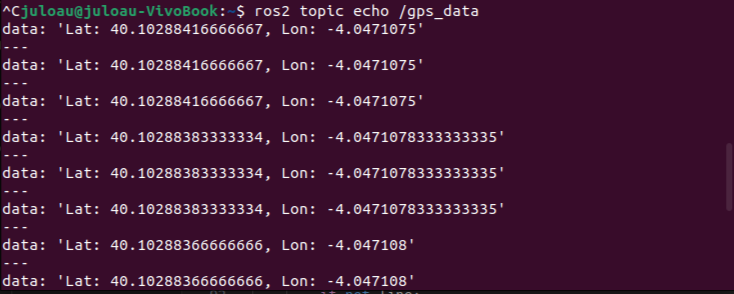
\includegraphics[width=12cm]{figs/cap6/echo_gps_controller.png}
	\end{center}
	\caption{Valores publicados de latitud y longitud captados del GPS}
	\label{fig:gpsnode}
\end{figure}


 \begin{figure} [h!]
	\begin{center}
		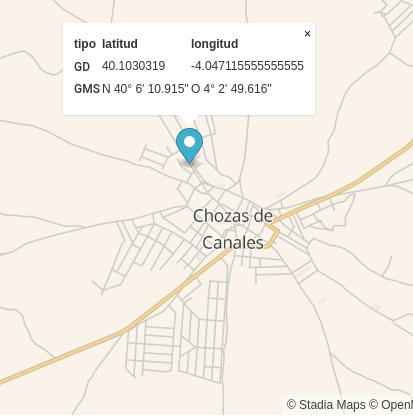
\includegraphics[width=15cm]{figs/cap6/localizacion.png}
	\end{center}
	\caption{Demostración de una correcta localización}
	\label{fig:demogpsnode}
\end{figure}

Debido a la distribución de Ubuntu usada, hay problemas con encender la Raspberry Pi si está conectado algo en el puerto serie\footnote{\url{https://wiki.ubuntu.com/EoanErmine/ReleaseNotes\#Raspberry_Pi}} pero las sugerencias no conseguían hacer funcionar bien el módulo; por lo tanto, la única solución encontrada fue desconectar el módulo \acs{GPS} hasta que se inicia sesión a través de ssh y luego conectar el módulo.

El módulo GPS realmente capta información válida cuando se enciende el LED azul que tiene integrado. Una forma fiable para que el módulo reciba todo el rato señal correcta es, dejarle en el exterior hasta que se encienda el LED y luego poder operar con el módulo en interior o exterior. 


\subsection{Motores}
\label{subsec:configmotores}


Explicar paso a paso y explicar y demostrar que todas las partes funcionan.

Seguí investigando y es importante tener en cuenta cómo funciona los servomotores, qué es la frecuencia y qué es PWM. (explicar todo eso del pwm... enlace: https://raspberrypi-espana.es/servo-frambuesa-pi/   más enlaces: https://www.youtube.com/watch?v=CHbUgggVQpA   otro enlace: https://solectroshop.com/es/blog/que-es-pwm-y-como-usarlo--n38)

Meter foto del movimiento de la rueda (que hice yo)


HUMBLE: detectar los pines -> añadir dialout a groups y hay que inicializar el demonio: sudo pigpiod

Contar lo de articulard robotics y que se intentó hacer ros2 control

\section{Software aplicado al robot físico}
\label{sec:softwarerf}

La idea era hacer un hardware interface pero no lo conseguí y decidí usar nodos publicadores y suscriptores.

COMENTAR TODO ESTE APARTADO A PARTIR DE LAS LÍNEAS DE CÓDIGO DE CADA FICHERO  




Capítulo 6: incluir lo de openvision paper\\

\subsection{Modelo Pin Hole}
\label{subsec:softwarepinhole}

Enlace donde se encuentra toda la información: https://github.com/RoboticsURJC/tfg-jlopez/wiki/Hip\%C3\%B3tesis-suelo

\subsection{Shoelace method}
\label{subsec:softwareshoelace}



Para calcular el área se ha decidido usar la fórmula "shoelace" (cordón de zapato). Es un algoritmo matemático para calcular el área de un polígono que se describe por sus coordenadas cartesianas (2D). El nombre de este algoritmo es debido a que tiene forma de atarse los cordones. Los puntos se tienen que colocar en sentido horario y el primer punto se tiene que duplicar y su segunda copia se sitúa al final de todos (como para cerrar el círculo).

Ejemplo de aplicación:

Cuadrado: (-140,-45), (-140,45), (140,45), (140,-45), (-140,-45)

Código en python:

def shoelace(coords):
n = len(coords)
area = 0.0

for i in range(n - 1):
x1, y1 = coords[i]
x2, y2 = coords[i + 1]
area += (x1 * y2) - (x2 * y1)

\# Agregar el último segmento
x1, y1 = coords[-1]
x2, y2 = coords[0]
area += (x1 * y2) - (x2 * y1)

return abs(area) / 2.0

El resultado es de 25200 mm²

La fórmula del rectángulo: base x altura

280*90 = 25200mm²

Coincide con la fórmula de "shoelace"

Algunas fuentes de información:

https://en.wikipedia.org/wiki/Shoelace\_formula

https://www.youtube.com/watch?v=iKIpraBC-Nw

https://www.youtube.com/watch?v=0KjG8Pg6LGk


Incluir lo del volumen medio de 40 mm de la RAC Foundation

\subsection{IA: yolov8 y aplicación a detectar baches}

\label{subsec:softwareiayolo}


Video de ultralytics que explica la instalación: https://www.youtube.com/watch?v=w4yHORvDBw0

Explicación del tipo de ia usada para este proyecto.

Tutoriales seguidos para conseguir el objetivo final: 

https://www.youtube.com/watch?v=1d\_JB-trK78

https://www.youtube.com/watch?v=XZ7FYAMCc4M


Inicialmente usaba LabelImg para definir dónde se encontraba los baches gracias a este tutorial he podido soclucionar un problema que tenía con este programa.  https://www.youtube.com/watch?v=5jHPuwo8z1o\&t=502s

AL FINAL USABA UN DATASET DE IMÁGENES CON MAYOR CANTIDAD PARA QUE LOS VALORES FUESEN MÁS EXACTOS

Guardé los datos como phdetect2.zip en Google Drive (que no acepta directamente subir un .zip y tuve que usar algún truquito) y gracias a seguir los pasos del tutorial2 en la parte de entrenarlo pude crear mi primera versión.


detect.tflite -> v1 usando CPU

detect\_edgetpu.tflite -> v1 convertida pero usa CPU

best\_....edge.tflite -> v2 muy pesada NO VA
bestv2.....edge.tflite -> v2 que sí va 

REVISAR NOMBRES 


Cuenta el paso a paso hasta conseguir la ia funcionando: https://github.com/RoboticsURJC/tfg-jlopez/wiki/Aprendizaje-Autom\%C3\%A1tico\#v2-de-la-ia-google-coral-usb-accelerator 

Explicacion de camera\_tfv3\_node (parte de tflite): https://github.com/RoboticsURJC/tfg-jlopez/wiki/Aprendizaje-Autom\%C3\%A1tico\#explicaci\%C3\%B3n-del-c\%C3\%B3digo (explica el código también. Fuente: https://www.youtube.com/watch?v=DGzQ7XIQyE8)


Explicar paso a paso el filtro de opencv para la detección correcta


TensorFlow Lite Inference

Sigue los siguientes pasos:

Cargar el .tflite modelo en memoria que contiene el grafo de ejecución del modelo

Transformar datos de la imagen para que sea compatible con el modelo .tflite

Hacer la inferencia. Este proceso sigue varios pasos como puede ser: crear un intérprete y fijar los tensores

Interpretar la salida según al gusto del desarrollador



CONTAR LO DE UPDATE EMA: https://admiralmarkets.com/es  (media movil exponencial)


\subsection{VFF}
\label{subsec:softwarevff}

Se ha usado la pendiente de la recta para hacer las conversiones .... Mirar los papeles y código: 

https://www.google.com/search?client=ubuntu-sn\&channel=fs\&q=pendiente+de+la+recta+\#vhid=HhxrPc0n8LdJsM\&vssid=l

Ejemplos en funcionamiento del vff:
https://gsyc.urjc.es/jmvega/research/webs/2019.html\#.21


Usar locks para evitar que haya condiciones de carrera: https://realpython.com/intro-to-python-threading/


Explicación del código que usa vff y desarrollé para rob servicios: https://robmovjuloau2022.blogspot.com/

\subsection{Interfaz Web}
\label{subsec:softwareweb}

O también conocido como HRI, se decidió usarla para facilitar el funcionamiento ...

Fuentes de información: 
https://en.wikipedia.org/wiki/Human\%E2\%80\%93robot\_interaction

https://journals.sagepub.com/doi/full/10.1177/0018720816644364


En Raspbian  hay que instalar apache... (como recordatorio, no incluirlo)


------ EN ROS2 HUMBLE --------------------------------------------------
He descubierto que en ros existe rosbridge\_server y trata de dar comunicación bidireccional entre clientes (buscadores web) y servidores usando una conexión Websocket. Para poder usarlo, primero hay que instalarlo y ejecutarlo en mi Raspberry:

sudo apt-get install ros-humble-rosbridge-suite
ros2 launch rosbridge\_server rosbridge\_websocket\_launch.xml

Para comprobar que escucha bien en el puerto 9090 rosbridge:

sudo lsof -i TCP:9090 | grep LISTEN

En otra terminal de la Raspberry , abre la ejecución del publicador del nodo gps:

source ./install/setup.bash
ros2 run pibotj\_rr gps\_node

En otra terminal de la Raspberry , crea un fichero .xml como este y ejecútalo en el directorio donde se encuentre (evita que sea dentro de ./src!!) de la siguiente forma:

python3 -m http.server 8000

En una nueva ventana del navegador insertar lo mismo que la imagen de abajo, cambiando la ip de tu raspberry.

Resultado final: Incluir imagen


\subsection{Detección de líneas}
\label{subsec:softwaredl}

Umbralización:  https://kipunaec.com/umbralizacion-o-thresholding-con-python-y-opencv/

\subsection{¿Aplicación Completa?}


¿Teleoperado y entorno controlado van en experimentos?



\section{Snippets}

Puede resultar interesante, para clarificar la descripción, mostrar fragmentos de código (o \textit{snippets}) ilustrativos. En el Código \ref{cod:codejemplo} vemos un ejemplo escrito en \texttt{C++}.

\begin{code}[h]
	\begin{lstlisting}[language=C++]
		void Memory::hypothesizeParallelograms () {
			for(it1 = this->controller->segmentMemory.begin(); it1++) {
				squareFound = false; it2 = it1; it2++;
				while ((it2 != this->controller->segmentMemory.end()) && (!squareFound)) {
					if (geometry::haveACommonVertex((*it1),(*it2),&square)) {
						dist1 = geometry::distanceBetweenPoints3D ((*it1).start, (*it1).end);
						dist2 = geometry::distanceBetweenPoints3D ((*it2).start, (*it2).end);
					}
					// [...]
				\end{lstlisting}
				\caption[Función para buscar elementos 3D en la imagen]{Función para buscar elementos 3D en la imagen}
				\label{cod:codejemplo}
			\end{code}
			
			En el Código \ref{cod:codejemplo2} vemos un ejemplo escrito en \texttt{Python}.
			
			\begin{code}[h]
				\begin{lstlisting}[language=Python]
					def mostrarValores():
					print (w1.get(), w2.get())
					
					master = Tk()
					w1 = Scale(master, from_=0, to=42)
					w1.pack()
					w2 = Scale(master, from_=0, to=200, orient=HORIZONTAL)
					w2.pack()
					Button(master, text='Show', command=mostrarValores).pack()
					
					mainloop()
				\end{lstlisting}
				\caption[Cómo usar un Slider]{Cómo usar un Slider}
				\label{cod:codejemplo2}
			\end{code}
			
			\section{Verbatim}
			
			Para mencionar identificadores usados en el código ---como nombres de funciones o variables--- en el texto, usa el entorno literal o verbatim \verb|hypothesizeParallelograms()|. También se puede usar este entorno para varias líneas, como se ve a continuación:
			
			\begin{verbatim}
				void Memory::hypothesizeParallelograms () {
					// add your code here
				}
			\end{verbatim}
			
			\section{Ecuaciones}
			
			Si necesitas insertar alguna ecuación, puedes hacerlo. Al igual que las figuras, no te olvides de referenciarlas. A continuación se exponen algunas ecuaciones de ejemplo: Ecuación \ref{ec:ec1} y Ecuación \ref{ec:ec2}.
			
			\begin{myequation}[h]
				\begin{equation}
					H = 1 - \frac{\sum_{i=0}^{N}\frac{(\frac{d_{j_s} + d_{j_e}}{2})}{N}}{M}
					\nonumber
					\label{ec:ec1}
				\end{equation}
				\caption[Ejemplo de ecuación con fracciones]{Ejemplo de ecuación con fracciones}
			\end{myequation} 
			
			\begin{myequation}[h]
				\begin{equation}
					v(entrada)= \left\{
					\begin{array}{lcc}
						0 & \mbox{if} & \epsilon_t < 0.1\\
						K_p\cdot{(T_{t}-T)} & \mbox{if}& 0.1 \leq \epsilon_t < M_t\\
						K_p \cdot M_t & \mbox{if}& M_t < \epsilon_t
					\end{array}
					\right.
					\label{ec:ec2}
				\end{equation}
				\caption[Ejemplo de ecuación con array y letras y símbolos especiales]{Ejemplo de ecuación con array y letras y símbolos especiales}
			\end{myequation}
			
			\section{Tablas o cuadros}
			
			Si necesitas insertar una tabla, hazlo dígnamente usando las propias tablas de \LaTeX, no usando pantallazos e insertándolas como figuras... En el Cuadro \ref{cuadro:ejemplo} vemos un ejemplo.
			
			\begin{table}[H]
				\begin{center}
					\begin{tabular}{|c|c|}
						\hline
						\textbf{Parámetros} & \textbf{Valores} \\
						\hline
						Tipo de sensor & Sony IMX219PQ[7] CMOS 8-Mpx \\
						Tamaño del sensor & 3.674 x 2.760 mm (1/4" format) \\
						Número de pixels & 3280 x 2464 (active pixels) \\
						Tamaño de pixel & 1.12 x 1.12 um \\
						Lente & f=3.04 mm, f/2.0 \\
						Ángulo de visión & 62.2 x 48.8 degrees \\
						Lente SLR equivalente & 29 mm \\
						\hline
					\end{tabular}
					\caption{Parámetros intrínsecos de la cámara}
					\label{cuadro:ejemplo}
				\end{center}
			\end{table}
			
			En los textos puedes poner palabras en \textit{cursiva}, para aquellas expresiones en sentido \textit{figurado}, palabras como \textit{robota}, que está fuera del diccionario castellano, o bien para resaltar palabras de una colección: \textit{(a)} es la primera letra del abecedario, \textit{(b)} es la segunda, etc.\\
			
			Al poner las dos líneas del anterior párrafo, este aparecerá separado del anterior. Si no las pongo, los párrafos aparecerán pegados. Sigue el criterio que consideres más oportuno.
			
			\section{Segunda sección}
			\label{sec:segundaseccion}
			
			No olvides incluir imágenes y referenciarlas, como la Figura \ref{fig:roomba}.
			
			\begin{figure} [h!]
				\begin{center}
					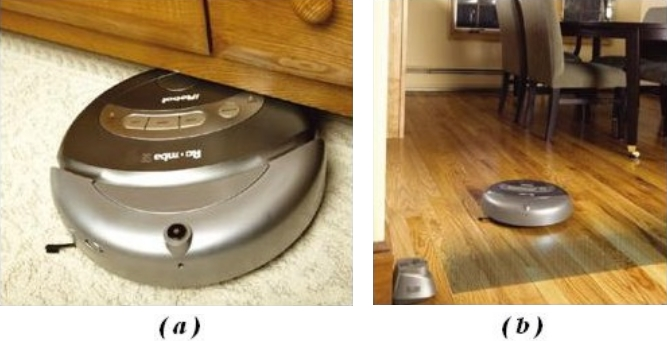
\includegraphics[width=8cm]{figs/roomba}
				\end{center}
				\caption{Robot aspirador Roomba de iRobot.}
				\label{fig:roomba}
			\end{figure}\
			
			Ni tampoco olvides de poner las URLs como notas al pie. Por ejemplo, si hablo de la Robocup\footnote{\url{http://www.robocup.org}}.
			
			\subsection{Números}
			\label{sec:subseccion}
			
			En lugar de tener secciones interminables, como la Sección \ref{sec:robotica}, divídelas en subsecciones.
			
			Para hablar de números, mételos en el entorno \textit{math} de \LaTeX, por ejemplo, $1.5Kg$. También puedes usar el símbolo del Euro como aquí: 1.500\euro.
			
			\subsection{Listas}
			
			Cuando describas una colección, usa \texttt{itemize} para ítems o \texttt{enumerate} para enumerados. Por ejemplo:
			
			\begin{itemize}
				\item \textit{Entorno de simulación.} Hemos usado dos entornos de simulación: uno en 3D y otro en 2D.
				\item \textit{Entornos reales.} Dentro del campus, hemos realizado experimentos en Biblioteca y en el edificio de Gestión.
			\end{itemize}\
			
			\begin{enumerate}
				\item Primer elemento de la colección.
				\item Segundo elemento de la colección.
			\end{enumerate}\
			
			\paragraph{Referencias bibliográficas}
			\label{sec:referencias}
			
			Cita, sobre todo en este capítulo, referencias bibliográficas que respalden tu argumento. Para citarlas basta con poner la instrucción \verb|\cite| con el identificador de la cita. Por ejemplo: libros como \cite{vega12e}, artículos como \cite{vega19b}, URLs como \cite{vega19a}, tesis como \cite{vega18b}, congresos como \cite{vega18a}, u otros trabajos fin de grado como \cite{vega08b}.
			
			Las referencias, con todo su contenido, están recogidas en el fichero \texttt{bibliografia.bib}. El contenido de estas referencias está en formato \texttt{BibTex}. Este formato se puede obtener en muchas ocasiones directamente, desde plataformas como \texttt{Google Scholar} u otros repositorios de recursos científicos.
			
			Existen numerosos estilos para reflejar una referencia bibliográfica. El estilo establecido por defecto en este documento es APA, que es uno de los estilos más comunes, pero lo puedes modificar en el archivo \texttt{memoria.tex}; concretamente, cambiando el campo \verb|apalike| a otro en la instrucción \verb|\bibliographystyle{apalike}|. 
			
			\
			
			\
			
			\
			
			Y, para terminar este capítulo, resume brevemente qué vas a contar en los siguientes.


\section{Corrector ortográfico}

Una vez tengas todo, no olvides pasar el corrector ortográfico de \LaTeX a todos tus ficheros \textit{.tex}. En \texttt{Windows}, el propio editor \texttt{TeXworks} incluye el corrector. En \texttt{Linux}, usa \texttt{aspell} ejecutando el siguiente comando en tu terminal:

\begin{verbatim}
aspell --lang=es --mode=tex check capitulo1.tex
\end{verbatim}
